% !TEX TS-program = pdflatex
% !TEX encoding = UTF-8 Unicode

% This is a simple template for a LaTeX document using the "article" class.
% See "book", "report", "letter" for other types of document.

\documentclass[10pt]{article} % use larger type; default would be 10pt

\usepackage[utf8]{inputenc} % set input encoding (not needed with XeLaTeX)

%%% Examples of Article customizations
% These packages are optional, depending whether you want the features they provide.
% See the LaTeX Companion or other references for full information.

%%% PAGE DIMENSIONS
\usepackage{geometry} % to change the page dimensions
\geometry{letterpaper} % or letterpaper (US) or a5paper or....
\geometry{margin=1in} % for example, change the margins to 2 inches all round
% \geometry{landscape} % set up the page for landscape
%   read geometry.pdf for detailed page layout information

\usepackage{graphicx} % support the \includegraphics command and options
\usepackage{mathrsfs}
% \usepackage[parfill]{parskip} % Activate to begin paragraphs with an empty line rather than an indent

%%% PACKAGES
\usepackage{booktabs} % for much better looking tables
\usepackage{array} % for better arrays (eg matrices) in maths
\usepackage{paralist} % very flexible & customisable lists (eg. enumerate/itemize, etc.)
\usepackage{verbatim} % adds environment for commenting out blocks of text & for better verbatim
\usepackage{subfig} % make it possible to include more than one captioned figure/table in a single float
\usepackage[font=small,labelfont=bf]{caption} % Required for specifying captions to tables and figures
% These packages are all incorporated in the memoir class to one degree or another...

%%% HEADERS & FOOTERS
\usepackage{fancyhdr} % This should be set AFTER setting up the page geometry
\pagestyle{fancy} % options: empty , plain , fancy
\renewcommand{\headrulewidth}{0pt} % customise the layout...
\lhead{}\chead{}\rhead{}
\lfoot{}\cfoot{\thepage}\rfoot{}

%%% SECTION TITLE APPEARANCE
\usepackage{sectsty}
\allsectionsfont{\sffamily\mdseries\upshape} % (See the fntguide.pdf for font help)
% (This matches ConTeXt defaults)

%%% ToC (table of contents) APPEARANCE
\usepackage[nottoc,notlof,notlot]{tocbibind} % Put the bibliography in the ToC
\usepackage[titles,subfigure]{tocloft} % Alter the style of the Table of Contents
\renewcommand{\cftsecfont}{\rmfamily\mdseries\upshape}
\renewcommand{\cftsecpagefont}{\rmfamily\mdseries\upshape} % No bold!
\newcommand{\centerfig}[2]{\begin{center}\includegraphics[width=#1\textwidth]{#2}\end{center}}
\usepackage{amssymb}
\usepackage{mathtools}
\DeclarePairedDelimiter\ceil{\lceil}{\rceil}
\DeclarePairedDelimiter\floor{\lfloor}{\rfloor}
\let\oldemptyset\emptyset
\let\emptyset\varnothing
\usepackage[usenames, dvipsnames]{color}
\makeatletter
\def\@maketitle{%
  \newpage
  \null
  \vskip 1em%
  \begin{center}%
  \let \footnote \thanks
	\vskip -5em%
    {\LARGE \@title \par}%
    \vskip 1em
    {\large
      \lineskip .5em%
      \begin{tabular}[t]{c}%
        \@author
      \end{tabular}\par}%
    \vskip 1em%
    {\large \@date}%
  \end{center}%
  \par
  \vskip 1.5em}
\makeatother
%%% END Article customizations

%%% The "real" document content comes below...

\title{Physics 410: Homework 2}
\author{Arnold Choa -- 32038144}
\date{12 October, 2018} % Activate to display a given date or no date (if empty),
         % otherwise the current date is printed 
%{\color{red}{\normalsize{\textbf{TODO}}}} %TODO signage
\begin{document}
\maketitle
\vspace{-0.5cm}
\noindent \Large{Question 1}
\\ \\
\normalsize{Please see \texttt{q1.py} in the \texttt{code} folder for the relevant code.}
\\ \\
\noindent \large{Part 1}
\\ \\
\normalsize{Please see below for the values we got from Python. We note that, computationally, rational numbers that are not a factor of 2 are just hard for the computer to calculate. Case in point, even the 0.994 inputted, gets turned into a long string of floating points until a close enough factor of 2 is found. This is calculated until 15 significant digits}
\[
\begin{array}{c | c | c | c | c}
n & Exact & R & P & Q \\
\hline & & & & \\
0	&	0.5				&	0.993999999999999\ldots	 		&	1					&	1					\\
1	&	0.25				&	0.497000000000000			&	0.49699999999999\dots 		&	0.49699999999999\ldots 		\\
2	&	0.125				&	0.248500000000000			&	0.24550000000000			&	0.24250000000000			\\
3	&	0.0625			&	0.124250000000000			&	0.119750000000000		&	0.109250000000000		\\
4	&	0.03125			&	0.062125000000000			&	0.056875000000000		&	0.030625000000000		\\
5	&	0.015625			&	0.031062500000000			&	0.025437500000000		&	-0.032687500000000		\\
6	&	0.0078125			&	0.015531250000000			&	0.009718750000000		&	-0.112343750000000		\\
7	&	0.00390625			&	0.007765625000000			&	0.001859375000000		&	-0.248171875000000		\\
8	&	0.001953125		&	0.003882812500000			&	-0.002070312500000		&	-0.508085937500000		\\
9	&	0.0009765625		&	0.001941406250000			&	-0.004035156250000		&	-1.02204296875000		\\
10	&	0.00048828125		&	0.000970703125000			&	-0.005017578125000		&	-2.04702148437500		\\
11	&	0.000244140625		&	0.000485351562500			&	-0.005508789062500		&	-4.09551074218750		\\
12	&	0.0001220703125		&	0.000242675781250			&	-0.005754394531250		&	-8.19175537109380		\\
13	&	0.00006103515625		&	0.000121337890625			&	-0.005877197265625		&	-16.3838776855470		\\
14	&	0.000030517578125	&	0.0000606689453125			&	-0.0059385986328125		&	-32.7679388427737		\\
15	&	0.0000152587890625	&	0.00003033447265625			&	-0.00596929931640625		&	-65.5359694213870		\\
16	&	0.00000762939453125	&	0.000015167236328125			&	-0.00598464965820315		&	-131.071984710694		\\
17	&	0.000003814697265625	&	0.0000075836181640625			&	-0.00599232482910158		&	-262.143992355348		\\
18	&	0.0000019073486328125	&	0.00000379180908203125		&	-0.00599616241455077		&	-524.287996177676		\\
19	&	9.5367431640625E-7	&	0.00000189590454101562		&	-0.00599808120727536		&	-1048.57599808884
\end{array}
\]
\newpage
\noindent \large{Part 2}
\\ \\
\normalsize{We can observe, even on the table above, that both the exact and r sequences converge to 0. As for the p sequence, though this dips below $0$, it also converges, but to $-0.006$ (this was checked later up until n=199). Finally, for the q sequence, this does not only dip below $0$, this sequence is unstable!}
\centerfig{.7}{../figs/q1_error.png}
\captionof{figure}{Plot of errors for the different pertured sequence. The sequences' values were baselined with the Exact value. We can see that the perturbed q sequence's errors grew exponentially with each iteration.}
\newpage
\noindent \large{Part 3}
\\ \\
\normalsize{First, we have to solve the general forms of the sequences:}
\\ \\
\noindent For the r sequence, it is simply a geometric sequence:
\begin{equation}
	r_{n} = \frac{1}{2}r_{n-1} = 2^{-n}r_{0}
\end{equation}
\noindent For the p sequence, we can assume a general solution of $p_{n} = As^{n}_{1} + Bs^{n}_2$. We can thus make a characteristic formula. Given reccurent sequence:
\begin{equation}
	p_{n} = \frac{3}{2}p_{n-1} - \frac{1}{2}p_{n-2}
\end{equation}
\noindent We can retrieve the characteristic polynomial:
\begin{equation}
	s^{2} = \frac{3}{2}s - \frac{1}{2}
\end{equation}
with roots $s = 1, \frac{1}{2}$. We thus end up with the general solution: 
\begin{equation}
	p_{n} = A + B2^{-n}
\end{equation}
with initial conditions $p_0 = p_0$ and $p_1 = p_1$. Solving for $A$ and $B$:
\begin{equation}
	p_{n} = \left(2p_1 - p_0 \right) + \left( 2\left( p_0 - p_1 \right) \right)2^{-n}
\end{equation}
\noindent Finally, for the q sequence, we can again assume a general solution of $q_{n} = As^{n}_{1} + Bs^{n}_2$. We can thus make a characteristic formula. Given reccurent sequence:
\begin{equation}
	q_{n} = \frac{5}{2}q_{n-1} - q_{n-2}
\end{equation}
\noindent We can retrieve the characteristic polynomial:
\begin{equation}
	s^{2} = \frac{5}{2}s - 1
\end{equation}
with roots $s = 2, \frac{1}{2}$. We thus end up with the general solution: 
\begin{equation}
	q_{n} = 2^{n}A + B2^{-n}
\end{equation}
with initial conditions $q_0 = q_0$ and $q_1 = q_1$. Solving for $A$ and $B$:
\begin{equation}
	q_{n} = \left(\frac{2q_1 - q_0}{3} \right)2^{n} + \left( \frac{2\left( 2q_0 - q_1 \right)}{3} \right)2^{-n}
\end{equation}
Going back to our results, as $n \rightarrow \infty$:
\begin{itemize}
	\item $r_n \rightarrow 0$
	\item $p_n \rightarrow 2p_1 - p_0$. In our case, $p_n \rightarrow 2(0.497) - 1 = -0.006$
	\item $q_n \rightarrow sign\left(\frac{2q_1 - q_0}{3} \right) \infty$ where the sign function gives $1$ is positive, $0$ if zero, and $-1$ if negative. In our case, $\left(\frac{2q_1 - q_0}{3} \right) = -0.002$ and so $q_n \rightarrow -\infty$. Note, we go by  the convention that $0 \cdot \infty = 0$.
\end{itemize}
\newpage
\noindent \Large{Question 2}
\\ \\
\normalsize{Please see \texttt{q2.py} in the \texttt{code} folder for the relevant code.}
\\ \\
\noindent \large{Part 1}
\\ \\
\normalsize{Solving by Gaussian elimination:}
\[ 
\left[
\begin{array}{c c | c}
\frac{1}{2} & \frac{1}{3} & 1\\
& & \\
\frac{1}{3} & \frac{1}{4} & -8
\end{array}
\right]
\Rightarrow
\left[
\begin{array}{c c | c}
\frac{1}{2} & \frac{1}{3} & 1\\
& & \\
0 & \frac{1}{36} & -\frac{26}{3}
\end{array}
\right]
\Rightarrow
\left[
\begin{array}{c c | c}
\frac{1}{2} & 0 & 105\\
& & \\
0 & \frac{1}{36} & -\frac{26}{3}
\end{array}
\right]
\Rightarrow
\left[
\begin{array}{c c | c}
1 & 0 & 210\\
& & \\
0 & 1 & -312
\end{array}
\right]
\]
\[ 
\left[
\begin{array}{c c | c}
\frac{1}{2} & \frac{1}{3} & 1\\
& & \\
\frac{1}{3} & -\frac{1}{2} & -8
\end{array}
\right]
\Rightarrow
\left[
\begin{array}{c c | c}
\frac{1}{2} & \frac{1}{3} & 1\\
& & \\
0 & -\frac{13}{18} & -\frac{26}{3}
\end{array}
\right]
\Rightarrow
\left[
\begin{array}{c c | c}
\frac{1}{2} & 0 & -3\\
& & \\
0 & -\frac{13}{18} & -\frac{26}{3}
\end{array}
\right]
\Rightarrow
\left[
\begin{array}{c c | c}
1 & 0 & -6\\
& & \\
0 & 1 & 12
\end{array}
\right]
\]
Thus, for our first system of equations: $\left[\begin{array}{c} x \\ y \end{array}\right] = \left[\begin{array}{c} 210 \\ -312 \end{array}\right]$. As for our second system of equations: $\left[\begin{array}{c} x \\ y \end{array}\right] = \left[\begin{array}{c} -6 \\ 12 \end{array}\right]$.
\\ \\ \\
\noindent \large{Part 2}
\\ \\
\normalsize{We will change the top-right $\frac{1}{3}$ for both systems. Solving via Gaussian elimination:}
\[ 
\left[
\begin{array}{c c | c}
\frac{1}{2} & \frac{33}{100} & 1\\
& & \\
\frac{1}{3} & \frac{1}{4} & -8
\end{array}
\right]
\Rightarrow
\left[
\begin{array}{c c | c}
\frac{1}{2} & \frac{33}{100} & 1\\
& & \\
0 & \frac{3}{100} & -\frac{26}{3}
\end{array}
\right]
\Rightarrow
\left[
\begin{array}{c c | c}
\frac{1}{2} & 0 & \frac{289}{3}\\
& & \\
0 & \frac{3}{100} & -\frac{26}{3}
\end{array}
\right]
\Rightarrow
\left[
\begin{array}{c c | c}
1 & 0 & \frac{578}{3}\\
& & \\
0 & 1 & -\frac{2600}{9}
\end{array}
\right]
\]
\[ 
\left[
\begin{array}{c c | c}
\frac{1}{2} & \frac{33}{100} & 1\\
& & \\
\frac{1}{3} & -\frac{1}{2} & -8
\end{array}
\right]
\Rightarrow
\left[
\begin{array}{c c | c}
\frac{1}{2} & \frac{33}{100} & 1\\
& & \\
0 & -\frac{18}{25} & -\frac{26}{3}
\end{array}
\right]
\Rightarrow
\left[
\begin{array}{c c | c}
\frac{1}{2} & 0 & -\frac{107}{36}\\
& & \\
0 & -\frac{18}{25} & -\frac{26}{3}
\end{array}
\right]
\Rightarrow
\left[
\begin{array}{c c | c}
1 & 0 & -\frac{107}{18}\\
& & \\
0 & 1 & \frac{325}{27}
\end{array}
\right]
\]
Thus, for our perturbed first system of equations: $\left[\begin{array}{c} x \\ \\  y \end{array}\right] = \left[\begin{array}{c} \frac{578}{3} \\ \\ -\frac{2600}{9} \end{array}\right]$. As for our perturbed second system of equations: $\left[\begin{array}{c} x \\ \\ y \end{array}\right] = \left[\begin{array}{c} -\frac{107}{18} \\ \\ \frac{325}{27} \end{array}\right]$.
\\ \\
For relative error, we will use the formula:
\begin{equation}
\eta = \frac{|x - x_{approx}|}{|x|}
\end{equation}
where $x$ is a vector and $|x|$ denotes the length of said vector. Thus, for the relative error of the first system:
\begin{equation}
\eta_{first} = \frac{\left| \left[\begin{array}{c} 210 \\ -312 \end{array}\right] - \left[\begin{array}{c} \frac{578}{3} \\ \\ -\frac{2600}{9} \end{array}\right]\right|}{\left| \left[\begin{array}{c} 210 \\ -312 \end{array}\right]\right|} \approx \frac{\left| \left[\begin{array}{c} \frac{52}{3} \\ \\ -\frac{208}{9} \end{array}\right] \right|}{376.09} \approx \frac{28.89}{376.09} \approx 7.68\%
\end{equation}
As for the relative error for the second system:
\begin{equation}
\eta_{second} = \frac{\left| \left[\begin{array}{c} -6 \\ 12 \end{array}\right] - \left[\begin{array}{c} -\frac{107}{18} \\ \\ \frac{325}{27} \end{array}\right]\right|}{\left| \left[\begin{array}{c} -6 \\ 12 \end{array}\right]\right|} \approx \frac{\left| \left[\begin{array}{c} -\frac{1}{18} \\ \\ -\frac{1}{27} \end{array}\right] \right|}{13.42} \approx \frac{0.067}{13.42} \approx 0.50\%
\end{equation}
\newpage
\noindent \large{Part 3}
\\ \\
\normalsize{No. The determinant is not an adequate measure of ill-conditioning. As a counter-example, let's take $10^{-1}\boldsymbol{I}$ where $\boldsymbol{I}$ is a $1000x1000$ identity matrix. Though its determinant is very small ($10^{-1000}$ to be exact), any small pertubation to any entry will not cause a singularity.}
\\ \\
We have to take what is called a \textit{condition number} of the matrix. This is the ratio between the larget and smallest singular values (derived from singular value decomposition). The larger the condition number of the matrix, the more likely it is to be ill-conditioned.
\\ \\
Taking our systems, the first system has a condition number of $\approx 38$ while the second system has a condition number of $\approx 1$. This means that the first system is more ill-conditioned than the second.
\\ \\
\noindent \large{Part 4}
\begin{center}
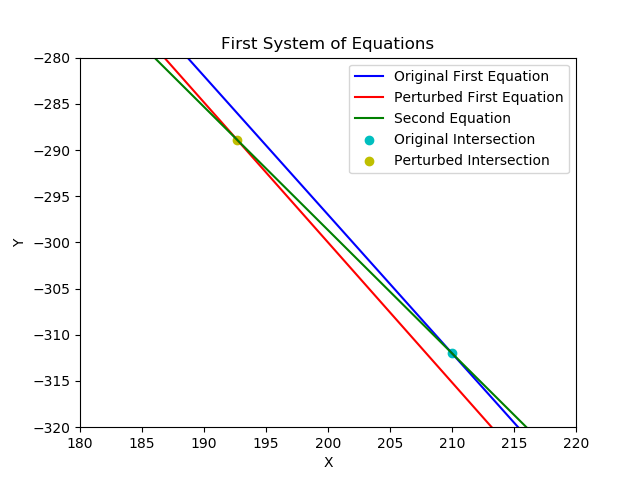
\includegraphics[width=.4\textwidth]{../figs/q2_first.png}
\captionof{figure}{Geometrical Representation of the first system of equations. We can see that the two lines are close to being colinear, and thus, any slight pertubation results in a massive change in the intersection.}
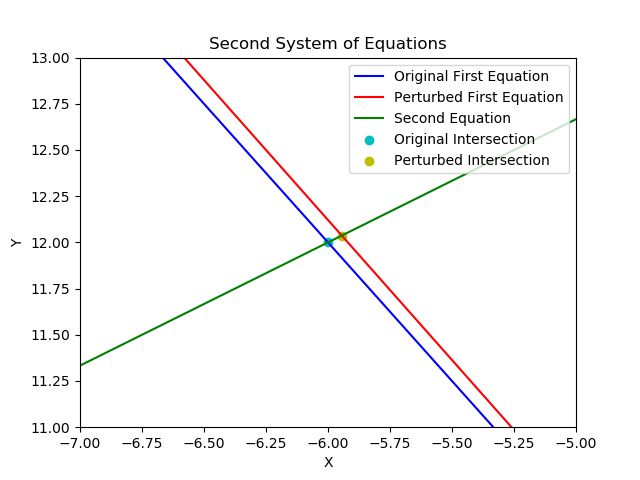
\includegraphics[width=.4\textwidth]{../figs/q2_second.png}
\captionof{figure}{Geometrical Representation of the second system of equations. We can see that the two lines are close to being perpendicula, and thus, any slight pertubation results in a very small change in the intersection.}
\end{center}
\normalsize{We can see more clearly, by using the geometrical representation, that the first system is very ill-conditioned as compared to the second. The major difference we can see from the two systems is that the ill-conditioned system is more colinear than the second (which is close to being orthogonal). Thus, given a slight pertubation to either equation, the first intersection of the first system will move wildly while the intersection of the second system will barely move at all, something  that we have seen in the relative errors generated above.}
\end{document}
